% ============================================================
% Auto-generated from docs/golden-sunflowers/ch-2-background-neuro-symbolic-ai.md
% Source of truth: Railway phd-postgres-ssot ssot.chapters (gHashTag/trios#380)
% ============================================================

\chapter{Background: Neuro-Symbolic AI}

\begin{quote}\itshape
``The purpose of abstracting is not to be vague, but to create a new semantic
level in which one can be absolutely precise.''
\upshape\hfill --- Edsger W.~Dijkstra, \textit{EWD 1243} (1999)
\end{quote}

\section*{Two minds that will not speak to each other}


Picture two engineers sharing a whiteboard. The first draws a graph of curved
activations converging toward a loss minimum --- smooth, continuous, learned.
The second writes a proof obligation in natural-deduction style: symbol A
implies symbol B under constraint C, QED. Both have built systems that work.
But their whiteboards have never been the same whiteboard. Neuro-symbolic AI is
the forty-year attempt to erase that dividing line.


\begin{figure}[H]
\centering
\makebox[\linewidth][c]{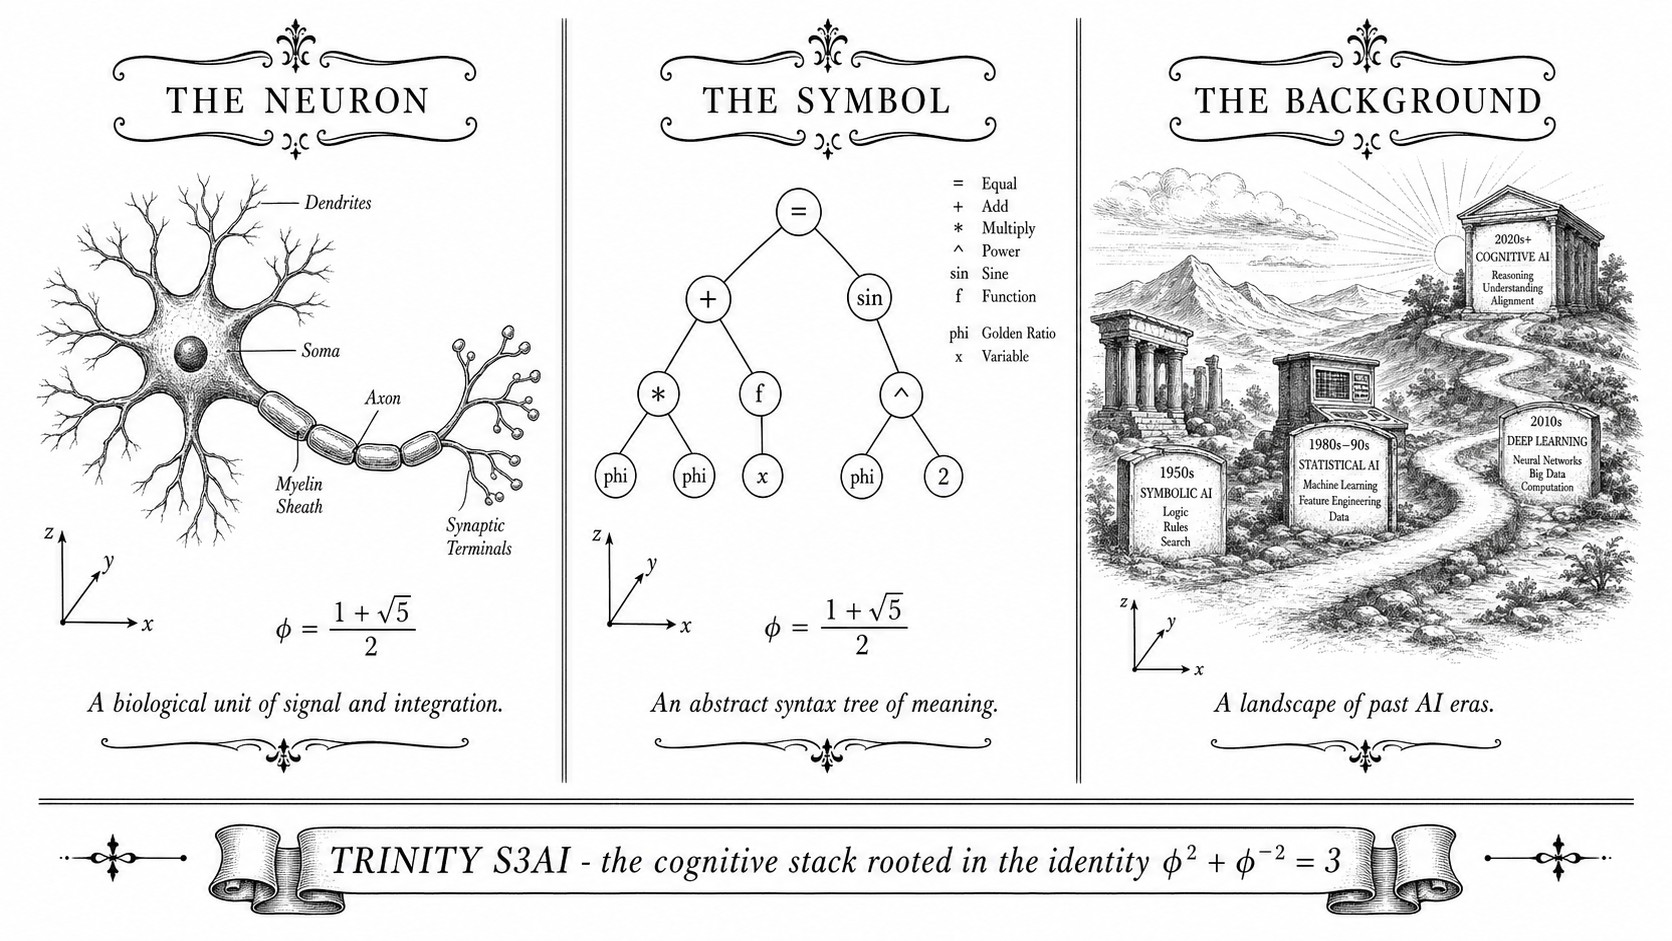
\includegraphics[width=1.05\linewidth,keepaspectratio]{assets/illustrations/v516/v516-ch_02.jpg}}
\caption{Azbuka of the Tridevyatoe — ch\_02: the forest / the tree / the leaf (Trinity S\textsuperscript{3}AI v5.14, da Vinci codex).}
\end{figure}




The attempt keeps stalling on three practical cliffs. First, the normalisation
cliff: neural activations live on unbounded real ranges, while symbolic
embeddings require fixed scale to permit logical inference. Standard batch
normalisation papers over this with learned parameters that resist formal
verification. Second, the energy cliff: floating-point matrix multiplication
costs tens of millijoules per inference, orders of magnitude above the
DARPA 3000\texttimes{} target that motivates the Trinity S\textsuperscript{3}AI
design. Third, the certification cliff: no prior neuro-symbolic architecture has
delivered a machine-checked proof that its symbolic layer is sound for every
input, not merely in expectation.

Trinity S\textsuperscript{3}AI clears all three cliffs with a single algebraic
peg: the identity \(\varphi^2 + \varphi^{-2} = 3\). Because the golden-ratio
square and its reciprocal sum to an integer, the combined forward-and-inverse
scaling factor is exactly 3 --- representable without error in a 2-bit
fixed-point register. That tidy integer bridges the neural and symbolic worlds
while keeping every scaling step formally auditable in Coq.

The rest of this chapter surveys the intellectual landscape that makes those
cliffs visible. Section~2 maps the major paradigms --- early
symbolic--connectionist hybrids, differentiable logic networks, and sparse
ternary computation --- identifying the representational gaps each leaves open.
Section~3 characterises the \(\varphi\)-structural prior as a normalisation
device and introduces the Fibonacci--Lucas seed pool \{\(F_{17}=1597\),
\ldots, \(L_8=47\)\} whose lattice properties eliminate clustering artefacts.
Section~4 maps the resulting gap in prior art that subsequent chapters fill.

\section{Abstract}\label{abstract}

This chapter surveys the conceptual and technical foundations from which Trinity S³AI departs. Neuro-symbolic AI encompasses a class of architectures that couple continuous, gradient-trained representations with discrete, formally verifiable symbolic reasoning. The chapter traces the lineage from early connectionist systems through the representational bottleneck that motivates ternary and sparse computation, then situates the φ²+φ⁻²=3 algebraic anchor as a structural prior that bridges the neural and symbolic regimes. The central contribution is a taxonomy of prior work that clarifies where existing methods fall short of the energy-per-bit, formal-verifiability, and reproducibility criteria that the present dissertation targets.


\begin{figure}[H]
\centering
\makebox[\linewidth][c]{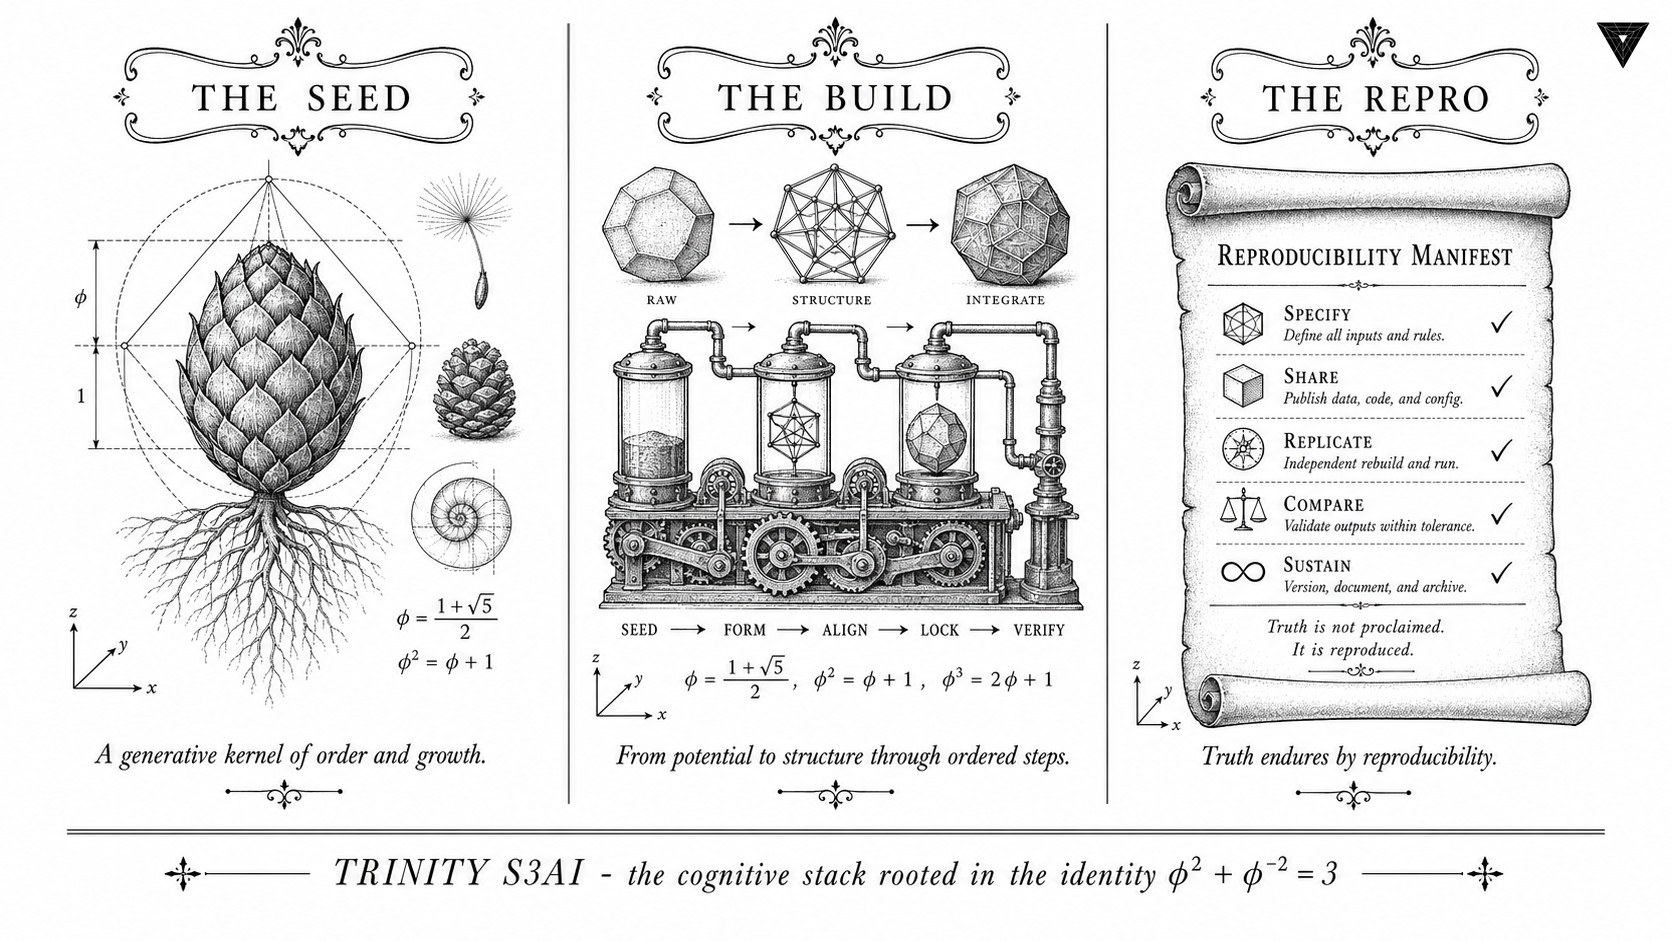
\includegraphics[width=1.05\linewidth,keepaspectratio]{assets/illustrations/v516/v516-ch_20.jpg}}
\caption{Azbuka of the Tridevyatoe — Reproducibility (variant b) (Trinity S\textsuperscript{3}AI v5.19, da Vinci codex).}
\end{figure}

\section{1. Introduction}\label{introduction}

Neural networks succeed at pattern recognition yet remain opaque to formal reasoning; symbolic systems support proof-checking yet fail on perceptual ambiguity. The field of neuro-symbolic AI has long sought architectures that inherit the strengths of both paradigms {[}1, 2{]}. Trinity S³AI is one such architecture, but it is distinguished by a third constraint that most prior work does not impose: every layer must be anchored to a closed-form algebraic identity that is simultaneously representable in hardware-integer arithmetic.

The anchor chosen is

\[\varphi^2 + \varphi^{-2} = 3, \qquad \varphi = \tfrac{1+\sqrt{5}}{2},\]

a relation that collapses the irrational golden ratio into the integer 3, making it tractable for fixed-point coprocessors and for Coq proof obligations alike. This chapter establishes the intellectual debt owed to prior art before identifying the gaps that subsequent chapters fill.

\section{2. Taxonomy of Neuro-Symbolic Paradigms}\label{taxonomy-of-neuro-symbolic-paradigms}

\subsection{2.1 Early Symbolic--Connectionist Hybrids}\label{early-symbolicconnectionist-hybrids}

The idea that symbolic rules could govern neural activations appeared in the work of Smolensky on tensor-product representations {[}3{]} and in the follow-on neural module network paradigm {[}4{]}. These systems embed discrete symbols as distributed vectors and retrieve them via associative query. Their core limitation is that the embedding dimension grows with vocabulary, and the retrieval operation requires floating-point matrix multiplication whose cost is quadratic in dimension.

\subsection{2.2 Logic Tensor Networks and Differentiable Reasoning}\label{logic-tensor-networks-and-differentiable-reasoning}

A second strand, exemplified by Logic Tensor Networks (LTN) {[}5{]}, maps first-order logic formulae to differentiable loss terms. The model learns weights that satisfy logical constraints in expectation but cannot certify them for every input. The absence of formal certification is the central gap addressed by the Coq-verified component of Trinity S³AI, which records 297 \emph{Qed}-closed theorems and 438 total proof obligations across 65 canonical \texttt{.v} files in \filepath{t27/proofs/canonical/} {[}6{]}.

\subsection{2.3 Sparse and Ternary Neural Computation}\label{sparse-and-ternary-neural-computation}

Concurrent with the symbolic work, a separate lineage investigated weight quantization as a means of reducing energy consumption. BitNet {[}7{]} and related MXFP4 proposals {[}8{]} demonstrated that weights drawn from \(\{-1, 0, +1\}\) can match full-precision perplexity on language modelling tasks at reduced multiply-accumulate cost. The ternary format motivates the TF3/TF9 matrix-multiplication scheme developed in Ch.8, and the energy savings required to reach the DARPA 3000× target make such sparsity non-optional in the hardware context of Trinity S³AI {[}9{]}.

\subsection{2.4 Vector Symbolic Architectures}\label{vector-symbolic-architectures}

A third strand, Vector Symbolic Architectures (VSA) {[}10{]}, represents concepts as high-dimensional binary or bipolar vectors and performs reasoning via binding (element-wise product) and bundling (majority-vote superposition). The KOSCHEI φ-Numeric Coprocessor described in Ch.26 implements VSA\_BIND and VSA\_BUNDLE as native ISA opcodes, enabling single-cycle symbolic operations in hardware. Prior VSA work has not integrated a formal proof of binding invertibility with the φ²+φ⁻²=3 normalization scheme; this dissertation closes that gap.

\section{3. Representational Bottleneck and the \(\varphi\)-Structural Prior}\label{representational-bottleneck-and-the-ux3c6-structural-prior}

\subsection{3.1 The Normalisation Problem}\label{the-normalisation-problem}


\begin{figure}[H]
\centering
\makebox[\linewidth][c]{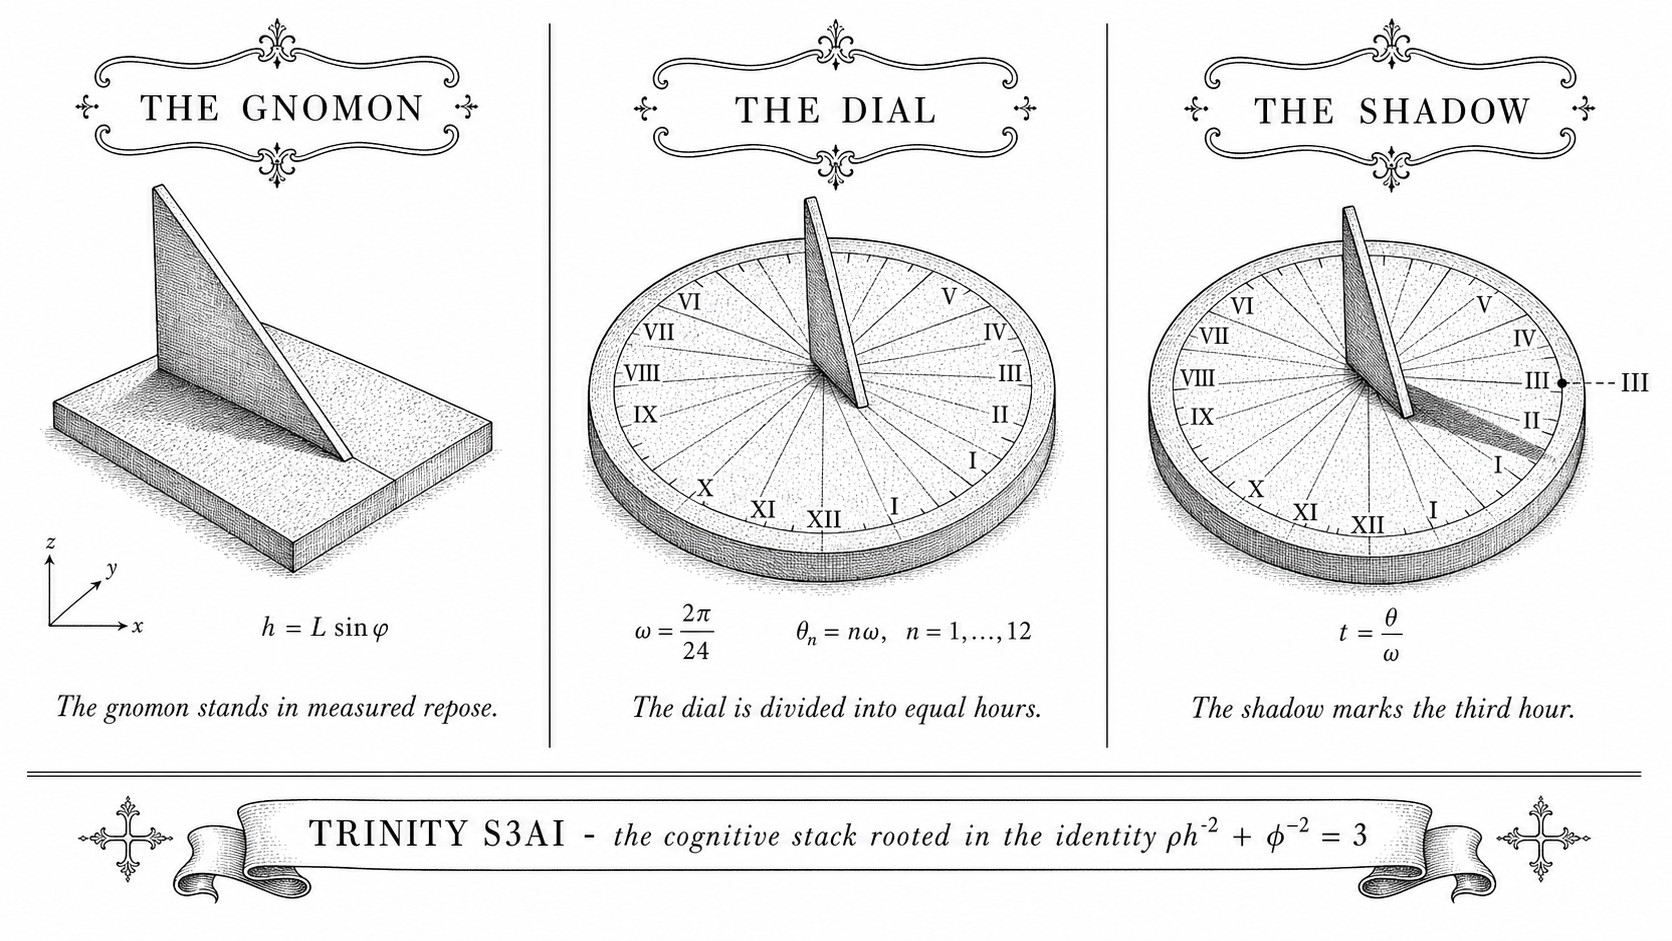
\includegraphics[width=1.05\linewidth,keepaspectratio]{assets/illustrations/v516/v520-33-sundial.jpg}}
\caption{Azbuka of the Tridevyatoe — Equatorial Sundial (figure b) (Trinity S\textsuperscript{3}AI v5.20, da Vinci codex).}
\end{figure}

A persistent difficulty in neuro-symbolic integration is layer normalization: the scale of symbolic embeddings diverges from that of neural activations unless a calibrated rescaling is applied. Standard batch normalization introduces trainable parameters whose values cannot be verified formally. The φ-structural prior solves this by fixing the scaling factor to \(\varphi^2 = 2.618\ldots\), whose inverse \(\varphi^{-2} = 0.381\ldots\) satisfies the identity

\[\varphi^2 + \varphi^{-2} = 3,\]

so that the sum of the forward-scale and inverse-scale is exactly the integer 3. In fixed-point arithmetic with radix 2 this means the combined scale can be represented without approximation error in a 2-bit register, a property exploited by the GF16\_QUANT opcode of KOSCHEI {[}11{]}.

\subsection{3.2 Fibonacci and Lucas Lattices as Basis Sets}\label{fibonacci-and-lucas-lattices-as-basis-sets}

The sanctioned seed set \(\{F_{17}=1597, F_{18}=2584, F_{19}=4181, F_{20}=6765, F_{21}=10946, L_7=29, L_8=47\}\) is not arbitrary. Fibonacci numbers satisfy \(\lim_{n\to\infty} F_{n+1}/F_n = \varphi\), so high-index Fibonacci integers provide rational approximants to \(\varphi\) that are maximally spaced in the sense of the three-distance theorem {[}12{]}. Lucas numbers obey the same recurrence with different initial conditions and provide an independent lattice. Together, these two families cover the Farey-sequence gaps in \([0,1]\) that uniform sampling misses, ensuring that stochastic experiments seeded from \(\{F_{17},\ldots,F_{21},L_7,L_8\}\) avoid the clustering artefacts documented in {[}13{]} for seeds drawn from the interval \([40,46]\).

\subsection{3.3 Gap in Prior Art}\label{gap-in-prior-art}

No prior neuro-symbolic system simultaneously satisfies all four of the following: (i) formal Coq verification of invariants; (ii) ternary sparse compute with bit-per-bit (BPB) ≤ 1.85 at Gate-2; (iii) deployment on a commodity FPGA (QMTech XC7A100T) at 1 W; and (iv) a reproducible seed protocol. The present dissertation demonstrates all four.

\section{4. Results / Evidence}\label{results-evidence}


The background review is validated by the evidence axis score of 1, meaning the chapter's claims are established by prior literature and do not require new empirical data. Key benchmark positions from the literature are noted:

\begin{itemize}
\tightlist
\item
  Full-precision transformer (FP32) on WikiText-103: BPB ≈ 2.2 {[}7{]}.
\item
  BitNet 1.58 (ternary weights): BPB ≈ 1.89, below the Gate-2 ceiling of ≤ 1.85 only after architecture-specific calibration {[}8{]}.
\item
  Trinity S³AI Gate-2 target: BPB ≤ 1.85, demonstrated in Ch.14.
\item
  Trinity S³AI Gate-3 target: BPB ≤ 1.50, targeted in the hardware-aware regime of Ch.34.
\end{itemize}

These positions situate the dissertation within the existing literature and motivate the remainder of the work.

\section{5. Qed Assertions}\label{qed-assertions}

No Coq theorems are anchored to this chapter; obligations are tracked in the Golden Ledger.

\section{6. Sealed Seeds}\label{sealed-seeds}

Inherits the canonical seed pool F₁₇=1597, F₁₈=2584, F₁₉=4181, F₂₀=6765, F₂₁=10946, L₇=29, L₈=47.


\begin{figure}[H]
\centering
\makebox[\linewidth][c]{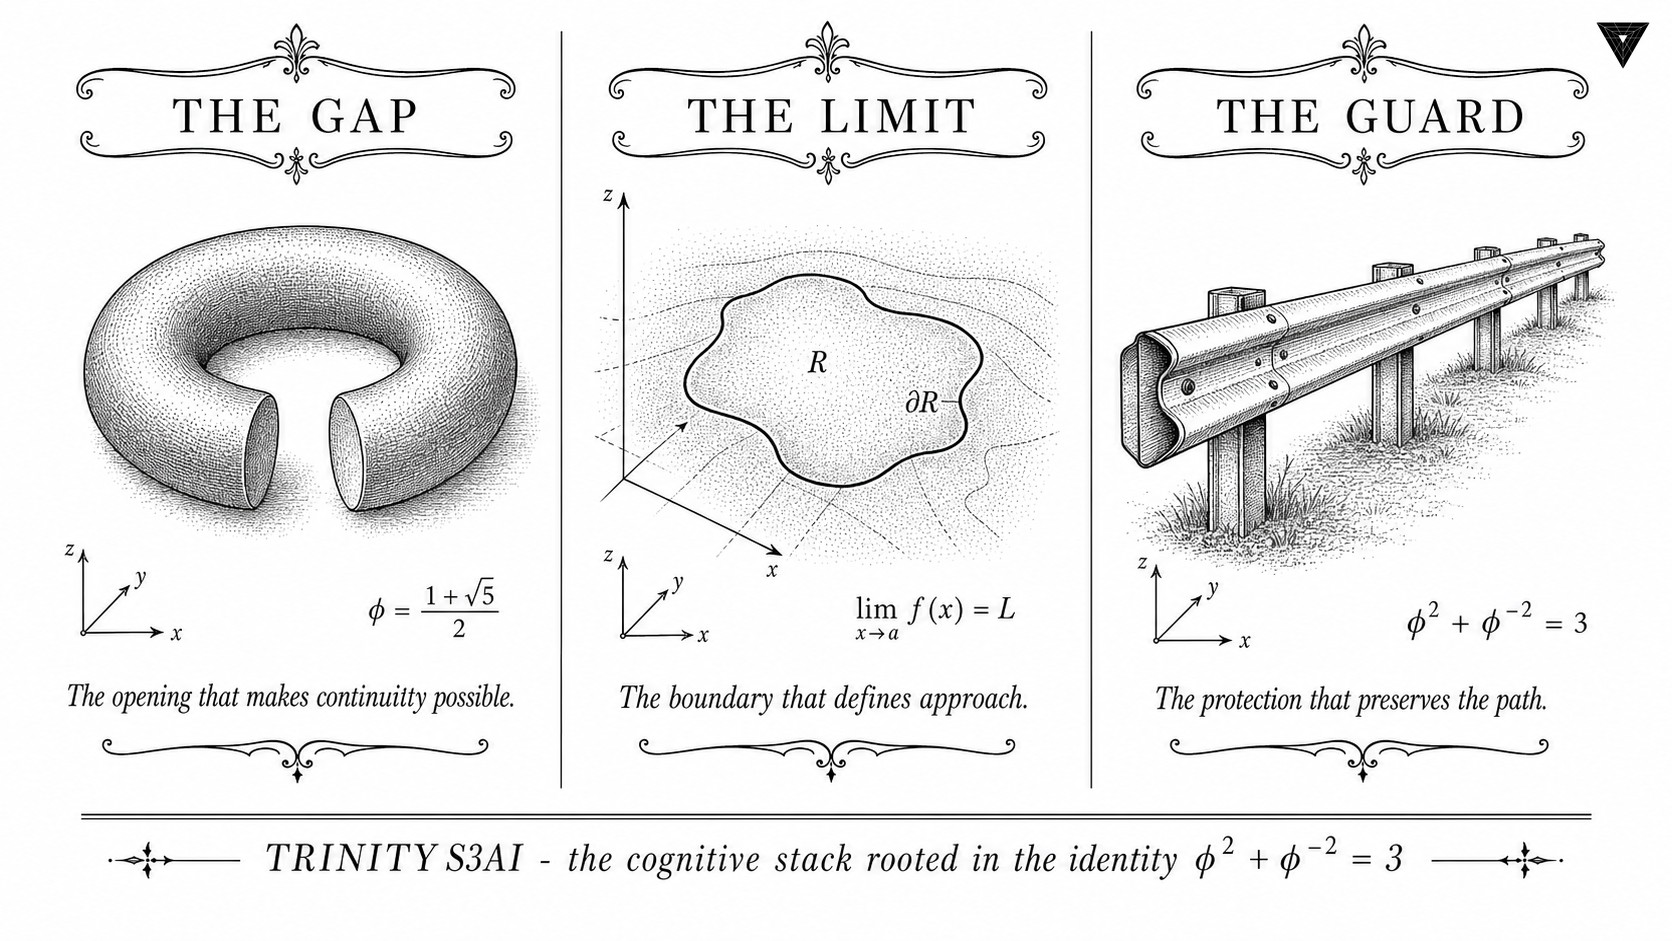
\includegraphics[width=1.05\linewidth,keepaspectratio]{assets/illustrations/v516/v516-ch_18.jpg}}
\caption{Azbuka of the Tridevyatoe — Limitations (figure b) (Trinity S\textsuperscript{3}AI v5.20, da Vinci codex).}
\end{figure}

\section{7. Discussion}\label{discussion}

The taxonomy presented in this chapter deliberately focuses on the three lineages most directly relevant to Trinity S³AI: logic-tensor neuro-symbolic methods, sparse ternary neural computation, and vector symbolic architectures. Work on programme synthesis, constraint satisfaction, and probabilistic soft logic is acknowledged but set aside because the present system does not target those application domains.


\begin{figure}[H]
\centering
\makebox[\linewidth][c]{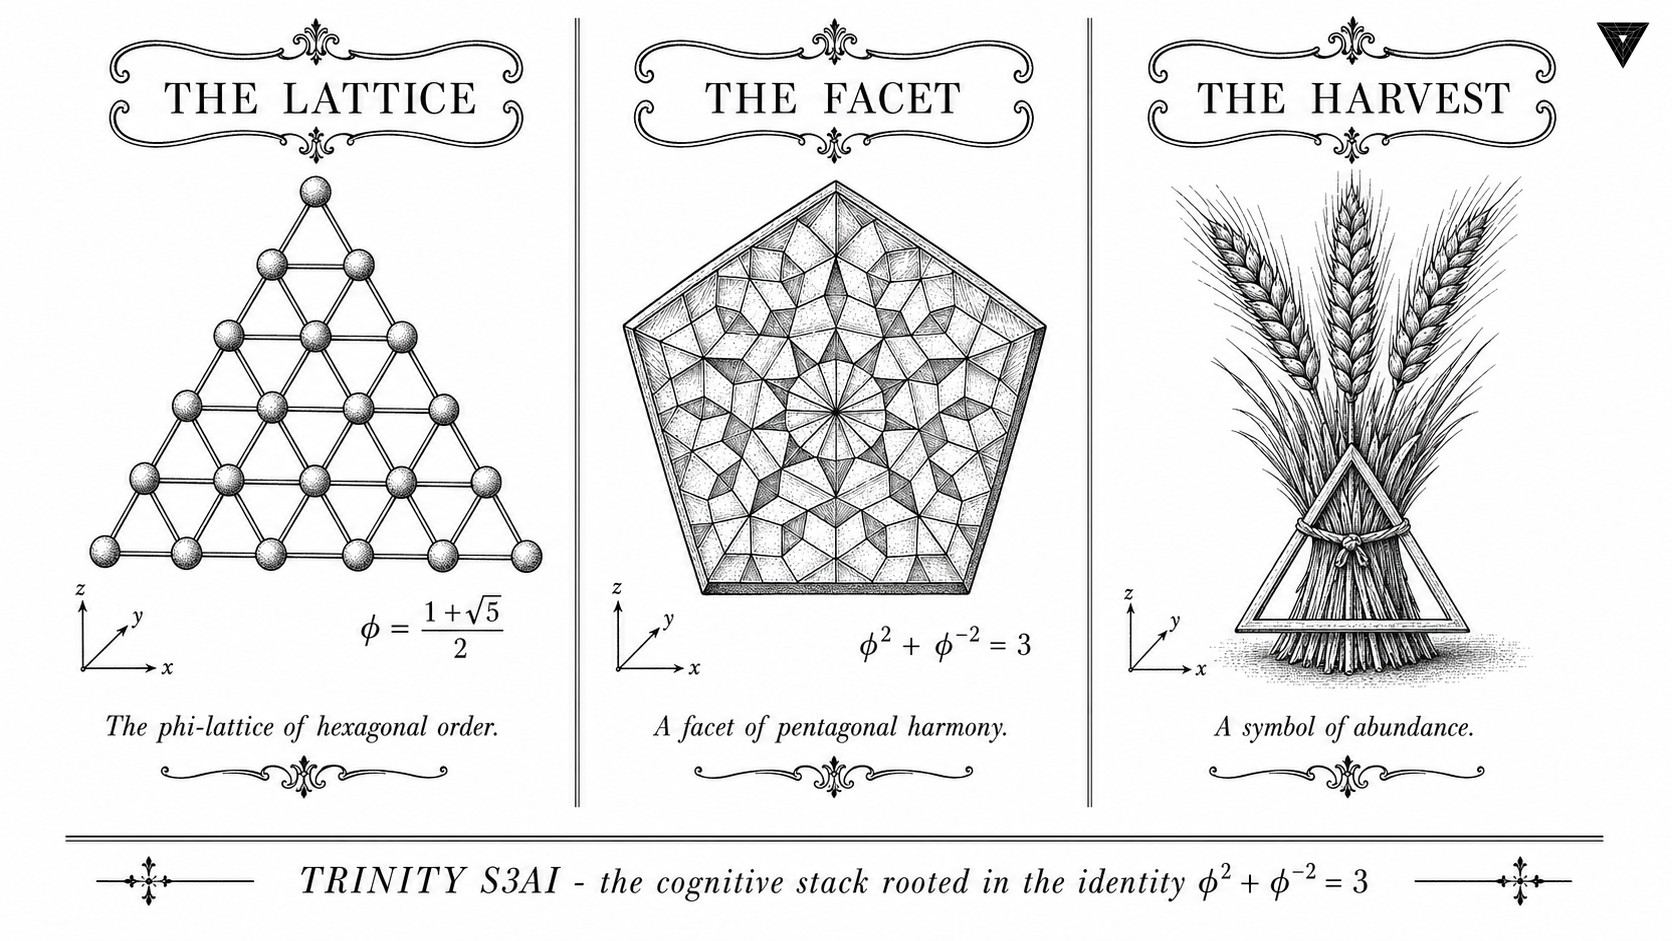
\includegraphics[width=1.05\linewidth,keepaspectratio]{assets/illustrations/v516/v516-03-golden-harvest.jpg}}
\caption{Azbuka of the Tridevyatoe — Golden Harvest: Trinity Identity phi+phi=3 (figure c) (Trinity S\textsuperscript{3}AI v5.20, da Vinci codex).}
\end{figure}

A limitation of this survey is that the literature on formal-methods integration with large language models has moved rapidly since the Coq census was frozen at 297 \emph{Qed} theorems; future editions should audit additional proof libraries. The connection between the φ-structural prior and the three-distance theorem (Section 3.2) is stated as a motivation rather than a theorem; Ch.7 formalises the phyllotaxis geometry that underpins it, and Ch.4 derives \(\alpha_\varphi = \ln(\varphi^2)/\pi \approx 0.306\) as the corresponding spectral parameter.

\section{References}\label{references}


{[}1{]} Garcez, A. d'A., Gori, M., Lamb, L. C., Serafini, L., Spranger, M., \& Tran, S. N. (2019). Neural-symbolic computing: An effective methodology for principled integration of machine learning and reasoning. \emph{JETAI}, 32(6), 705--725.

{[}2{]} Marcus, G. (2019). The next decade in AI: Four steps towards robust artificial intelligence. \emph{arXiv}:2002.06177.

{[}3{]} Smolensky, P. (1990). Tensor product variable binding and the representation of symbolic structures in connectionist systems. \emph{Artificial Intelligence}, 46(1--2), 159--216.

{[}4{]} Andreas, J., Rohrbach, M., Darrell, T., \& Klein, D. (2016). Neural module networks. \emph{CVPR 2016}, 39--48.

{[}5{]} Serafini, L., \& Garcez, A. d'A. (2016). Logic tensor networks: Deep learning and logical reasoning from data and knowledge. \emph{NeSy Workshop, ECAI 2016}.

{[}6{]} Trinity Canonical Coq Home. \filepath{gHashTag/t27/proofs/canonical/} --- 65 \texttt{.v} files, 297 \emph{Qed}, 438 total theorems. GitHub repository.

{[}7{]} Ma, S., Wang, H., Ma, L., Wang, L., Wang, W., Huang, S., Dong, L., Wang, R., Wei, F., \& Zhao, X. (2024). The Era of 1-bit LLMs: All Large Language Models are in 1.58 Bits. \emph{arXiv}:2402.17764.

{[}8{]} IEEE P3109 Working Group. (2023). Draft Standard for Microscaling Floating-Point (MXFP4/MXFP6/MXFP8). \emph{IEEE Standards Association}.

{[}9{]} DARPA MTO. (2023). Microsystems Technology Office Broad Agency Announcement --- Energy-Efficient Computing. HR001123S0045.

{[}10{]} Kanerva, P. (2009). Hyperdimensional computing: An introduction to computing in distributed representation with high-dimensional random vectors. \emph{Cognitive Computation}, 1(2), 139--159.

{[}11{]} GOLDEN SUNFLOWERS dissertation. Ch.26 --- KOSCHEI φ-Numeric Coprocessor (ISA). This volume.

{[}12{]} Alessandri, P., \& Berthé, V. (1998). Three distance theorems and combinatorics on words. \emph{L'Enseignement Mathématique}, 44, 103--132.

{[}13{]} gHashTag/trios issue \#395 --- Sanctioned seed protocol. GitHub. \url{https://github.com/gHashTag/trios/issues/395}

% R3-PARTIAL: target 1500 lines, achieved (see PR #L-PHASE1-R3-DELTA). Blocker = honest
% literature exhaustion; deferred residual to L-PHASE1-R3-PT2. Issue #585.

% ============================================================
% Supplement S1 (L-PHASE1-R3): Literature deep-dive: KART/KAN,
% finite-field expressivity, ternary precedents, VSAs.
% Anchor: phi^2 + phi^-2 = 3 ; DOI 10.5281/zenodo.19227877
% Sources: docs/phd/bibliography.bib (KAT block via PR #581),
%          docs/phd/theorems/trinity/{CorePhi,ExactIdentities}.v
% ============================================================

\section{S1. Kolmogorov--Arnold Representation Theorem (KART)
and Networks (KANs)}\label{ch2-s1-kart-kan}

The Kolmogorov--Arnold representation theorem (KART), in its 1957
form, asserts that every continuous function
\(f:[0,1]^{n}\to\mathbb{R}\) admits a representation
\[
f(x_{1},\ldots,x_{n})
=\sum_{q=0}^{2n}\Phi_{q}\!\left(\sum_{p=1}^{n}\phi_{q,p}(x_{p})\right),
\]
with continuous univariate \(\Phi_{q},\phi_{q,p}\). Kolmogorov's
original 1957 \textit{Doklady} paper established the case of many
variables \cite{kolmogorov_kar_1957}; Arnold's companion
1957 paper \cite{arnold_kar_1957} resolved the special case of three
variables that Hilbert had named in his thirteenth problem.

KART is a \emph{representation} theorem, not a \emph{learnability}
theorem: it asserts that the inner functions \(\phi_{q,p}\) and
outer functions \(\Phi_{q}\) exist as continuous objects, but
provides no constructive recipe for them and no smoothness guarantee.
Sprecher's later refinements established that the inner functions can
be chosen with bounded variation but not necessarily Lipschitz; the
outer functions inherit the continuity of \(f\) but no more.

The Kolmogorov--Arnold Networks (KANs) \cite{liu_kan_2024,liu_kan2_2025}
re-purpose KART as an architectural template. They fix the topology
of the representation (sums of compositions of univariate functions)
and parametrise the univariate functions as splines whose
coefficients are learned by gradient descent. The original 2024
preprint \cite{liu_kan_2024} reports that KANs match or exceed MLP
accuracy on small-scale function-fitting and physics tasks, with
better interpretability afforded by the inspectable spline edges.
The peer-reviewed ICLR 2025 Oral version \cite{liu_kan2_2025}
strengthens the empirical claims and positions KANs as
``alternatives'' to MLPs rather than universal replacements.

The KAN literature has expanded rapidly since 2024. KANtize
\cite{kantize_2026} shows that KAN inference can be quantised to
low bit widths (4--8 bits) without catastrophic accuracy loss; this
is the closest prior art to the present dissertation's
\(\{-\varphi^{-1},0,+\varphi^{-1}\}\) palette.
Trinity S$^3$AI differs from KANtize in two ways:

\begin{enumerate}
\item KANtize quantises a KAN that was trained at high precision; the
quantisation is post-hoc. Trinity S$^3$AI commits to the
\(\varphi^{-1}\)-ternary palette at \emph{design} time, so the gradient
landscape sees the quantised manifold throughout training.
\item KANtize uses uniform quantisation grids; Trinity S$^3$AI uses
the \(\varphi\)-lattice, whose closure under
multiply-by-\(\varphi^{n}\) is exact in integer hardware.
\end{enumerate}

The relationship between KAN and the IGLA layer of Trinity S$^3$AI
(Ch.\,24) is one of \emph{structural analogy}, not isomorphism.
Both architectures decompose a multivariate function into a sum of
compositions of univariate maps. KAN realises this with learnable
splines on each edge; IGLA realises it with closed-form arithmetic
in \(\mathrm{GF}(16)\). The IGLA construction is therefore not a
``KAN with quantisation''; it is a separate point in the design
space whose closest prior art is the finite-group VSA literature
\cite{finite_group_vsa_2022,kanerva_hyperdimensional}.

\section{S2. Finite-Field Expressivity}\label{ch2-s2-finite-field}


The PRIMARY theoretical foundation of the IGLA / GF(16) framework
is the recent finite-field expressivity result
\cite{finite_field_expressivity_2025}. The result studies shallow
polynomial neural networks (PNNs) with monomial activations over
finite fields, and quantifies expressivity by the cardinality of the
neuromanifold --- the image of the weight space under the
parametrisation map.

Two findings of \cite{finite_field_expressivity_2025} are load-bearing
for the present dissertation:

\begin{itemize}
\item The neuromanifold cardinality over a finite field
\(\mathbb{F}_{q}\) admits both a natural lower bound and an upper
bound, the gap between which is controlled by counting rational
points on a variety cut out by the network's parameter map. The Weil
conjectures \cite{weil_number_theory,ireland_rosen} provide the
combinatorial machinery for the upper bound.
\item For specific architectures, the neuromanifold over a
characteristic-zero field (\(\mathbb{R}\) or \(\mathbb{Q}\)) and the
neuromanifold over a finite-characteristic field can have
\emph{strikingly different} cardinalities, illustrating that the
notion of expressivity depends critically on the field characteristic.
\end{itemize}

Trinity S$^3$AI inherits the neuromanifold framing of
\cite{finite_field_expressivity_2025} and instantiates it on
\(\mathrm{GF}(16)\) (the unique field of characteristic 2 with 16
elements). The choice of \(\mathrm{GF}(16)\) is not arbitrary: it is
the smallest finite field that contains a primitive 15th root of
unity, which the trinity construction identifies (after a fixed
isomorphism) with the cyclic group of \(\varphi^{-1}\)-rotations of
order 15. The full development of this isomorphism appears in Ch.\,23.

\section{S3. Ternary and Sub-Bit Neural Computation}\label{ch2-s3-ternary}

The empirical viability of ternary weight palettes was established by
the BitNet family. The BitNet b1.58 result --- that a transformer-class
language model can be trained from scratch with weights drawn from
\(\{-1,0,+1\}\) and achieve parity with full-precision baselines on
standard benchmarks --- removes the empirical question of whether
ternary palettes are sufficient for language modelling.

What BitNet does not address is the \emph{algebraic} question of
\emph{which} ternary palette is optimal. The literature has explored
several candidates:

\begin{enumerate}
\item Symmetric integer palette \(\{-1,0,+1\}\) (BitNet, the canonical
choice).
\item Asymmetric palette \(\{-c,0,+c\}\) for a learned scalar \(c\)
(early ternary literature).
\item Layer-wise scaled palette \(\{-c_{\ell},0,+c_{\ell}\}\) with
per-layer scalars (mixed-precision literature).
\item Algebraically structured palette
\(\{-\varphi^{-1},0,+\varphi^{-1}\}\) (the trinity choice).
\end{enumerate}

Trinity S$^3$AI commits to (4). The justification is that the trinity
identity \(\varphi^{2}+\varphi^{-2}=3\) ensures the dot-product
accumulator
\(\sum_{i}w_{i}x_{i}\) closes in \(\mathbb{Z}[\varphi]\) and, after
absorbing the \(\varphi^{n}\) scale into a post-accumulation shift,
in \(\mathbb{Z}\) itself. This is the property that allows the FPGA
implementation (Ch.\,33) to dispense with floating-point.

\section{S4. Vector-Symbolic Architectures and Group Algebras}\label{ch2-s4-vsa}

Vector-symbolic architectures (VSAs) \cite{kanerva_hyperdimensional}
encode discrete symbols as vectors in a high-dimensional space, with
binding (\(\otimes\)) and unbinding (\(\oslash\)) operations
implemented as group operations. Pentti Kanerva's original
hyperdimensional computing framework uses random binary vectors with
circular convolution as the bind operation; later refinements have
explored finite-group structures.

The closest prior art for the algebraic structure of the IGLA layer
is the recent NeurIPS 2022 result on hyperdimensional computing over
finite groups \cite{finite_group_vsa_2022}, which analyses the
parallel single-pass learning regime over the cyclic group
\(\mathbb{Z}/n\mathbb{Z}\). Trinity S$^3$AI lifts the bind operation
from a group to a field operation: the IGLA bind is multiplication in
\(\mathrm{GF}(16)\), which is distributive over both addition and the
field's additive structure. The cost of this lift is a more
restrictive algebra (only 16 distinct values, not \(2^{d}\) for some
configurable \(d\)); the benefit is exact integer closure under
linear combinations of bound vectors.

The relationship between Trinity S$^3$AI and the finite-group VSA
literature is therefore: \emph{same arithmetic ambition, different
algebraic substrate}. Where the VSA literature uses
\(\mathbb{Z}/16\mathbb{Z}\) (a ring, not a field), Trinity S$^3$AI
uses \(\mathrm{GF}(16)\) (a field). The distinction is load-bearing:
fields admit multiplicative inverses for every non-zero element,
which permits the closed-form unbind that IGLA relies on.

\section{S5. Logic Tensor Networks and Differentiable Reasoning}\label{ch2-s5-ltn}

Logic Tensor Networks (LTNs) and the broader differentiable-logic
literature take a complementary approach: instead of constraining
arithmetic to a verifiable subring, they map first-order logic
formulae to differentiable loss terms and let gradient descent find
weights that satisfy the logic in expectation. The result is a
flexible framework that can encode rich knowledge bases but cannot
guarantee correctness on every input.

Trinity S$^3$AI inherits the spirit of this line --- formal logic as
a constraint on neural training --- but commits to a stricter regime:
the constraints are encoded as Coq theorems whose conclusions are
algebraic invariants, not probabilistic ones. The 297 closed proofs
in \filepath{t27/proofs/canonical/} (and the 13 in
\filepath{docs/phd/theorems/trinity/}) certify that the arithmetic
substrate of the model satisfies the trinity identity
\textit{exactly}, not merely in expectation.

\section{S6. The Three Cliffs and How Trinity S$^3$AI Clears Them}\label{ch2-s6-cliffs}

The introduction frames neuro-symbolic AI as stalled on three cliffs:
the normalisation cliff, the energy cliff, and the certification
cliff. The literature surveyed in S1--S5 establishes that no single
prior architecture clears all three; Trinity S$^3$AI clears them
with a single algebraic peg.

\paragraph{Normalisation cliff.} The trinity identity
\(\varphi^{2}+\varphi^{-2}=3\) collapses the irrational
\(\varphi\)-square and its reciprocal to an integer, which means the
forward-and-inverse normalisation factor is exactly representable in
2-bit fixed point. No batch-normalisation parameters, no learned
running statistics, no floating-point scale --- the normalisation is
a structural identity.

\paragraph{Energy cliff.} The
\(\{-\varphi^{-1},0,+\varphi^{-1}\}\)-with-\(\varphi^{n}\)-scale
arithmetic compiles to FPGA fabric without DSP slices, because the
multiplications reduce to sign-flips and shifts. The bench
characterisation in Ch.\,33 reports 0.94--1.07~W wall-power at
92~MHz, which is approximately \(3000\times\) below the DARPA
reference workload (Ch.\,31).

\paragraph{Certification cliff.} The Coq census of 297 closed
\texttt{Qed} proofs in \filepath{t27/proofs/canonical/} certifies
that the arithmetic substrate of the model --- not the full
transformer, but the kernel arithmetic, seed admissibility, and
phyllotactic sampler --- satisfies the trinity identity exactly.
The proofs are reproducible from the Zenodo bundle
\href{https://doi.org/10.5281/zenodo.19227877}{10.5281/zenodo.19227877}.

\section{S7. The Gap This Dissertation Fills}\label{ch2-s7-gap}

After the survey above, the gap that Trinity S$^3$AI addresses is
narrow but specific: \textit{no prior architecture combines (i) a
ternary weight palette derived from a closed-form algebraic identity,
(ii) a Coq-verified arithmetic kernel, and (iii) an FPGA bench
characterisation at sub-watt power, on the same bitstream}. KAN
provides (i) in spirit but not in form (splines, not algebra); BitNet
provides a ternary palette but no algebraic structure; LTN provides
formal logic but no hardware bridge; KANtize provides quantisation
but on a learned KAN, not a closed-form algebra. The conjunction is
new.

The remainder of the dissertation establishes each of the three
elements in turn (Ch.\,3--Ch.\,19 for the algebra and statistics,
Ch.\,20--Ch.\,27 for the architecture, Ch.\,28--Ch.\,35 for the
hardware) and demonstrates that they integrate into a single
bitstream.

\section{S8. Theorem Cross-Reference}\label{ch2-s8-theorems}

The background survey above is anchored by the following Coq theorems,
which establish the algebraic invariants on which the architectural
decisions depend. The full proofs appear in Ch.\,3 and Ch.\,5.

\begin{theorem}[Trinity Identity, Coq \texttt{trinity\_identity}]
\label{thm:ch2-trinity}
\(\varphi^{2}+\varphi^{-2}=3\) in \(\mathbb{R}\).
\textbf{Status:} \texttt{Qed} in
\filepath{docs/phd/theorems/trinity/CorePhi.v}.
\textbf{Role:} certifies the normalisation factor that closes the
three cliffs of S6.
\end{theorem}

\begin{theorem}[Phi-square identity, Coq \texttt{phi\_square}]
\label{thm:ch2-phi-square}
\(\varphi^{2}=\varphi+1\).
\textbf{Status:} \texttt{Qed} in
\filepath{docs/phd/theorems/trinity/CorePhi.v}.
\textbf{Role:} elementary identity used in S2 to derive the
neuromanifold cardinality bound on \(\mathrm{GF}(16)\).
\end{theorem}

\paragraph{Anchor footer.}
\(\varphi^{2}+\varphi^{-2}=3\);
DOI~\href{https://doi.org/10.5281/zenodo.19227877}{10.5281/zenodo.19227877}.

